\documentclass{article}
\usepackage{graphicx}
\usepackage{float}
\setlength{\parskip}{1.15ex}
\title{Modified Couzin Model: Collective Animal Behavior on different conditions}
\author{Kazi Nahid Reaz, Dilshad Jahan Rupa, Afsana Islam Mimi}
\date{August 25, 2017}


\begin{document}
\maketitle

\abstract{
This report indicates some interesting flocking behavior of animals based on different values on existing Couzin Model. In this experiment, we have found some interesting agents behavior that leads us to four interesting flocking patterns from the existing Couzin Model. It shows how the agents behave on different atmosphere or condition and how they change their moving ways depending on that.
}

\section{Introduction}

Couzin Model is a collective animal behavior model that shows  the behavior of animal flocking in different conditions. This model actually runs on two major rules. They are :
(1) Individuals attempt to maintain a minimum distance between themselves and others at all times. This rule has the highest priority and corresponds to a frequently observed behavior of animals in nature (Krause \& Ruxton, 2002).]
(2) If individuals are not performing an avoidance maneuver (rule 1) they tend to be attracted towards other individuals (to avoid being isolated) and to align themselves with neighbors (Partridge \& Pitcher, 1980; Partridge,1982). These behavioral tendencies are simulated using local perception and simple response behaviors.] [1]
Couzin model operates under following parameters - 
(1) Number of individuals
(2) Zone of repulsion
(3) Zone of orientation
(4) Zone of attraction
(5) Field of perception
(6) Turning rate
(7) Noise
Using these parameters this model indicates a three-dimensional animal flocking that actually reflects their real life behavior. 


\section{Methodology}
Our main objective was to find any different behavior of the agents so that we can identify and relate with the real life animal behavior. Firstly, we run the existing Couzin Model on different parameters through Behaviorsearch that provided us some data which enabled us to observe the differences between the existing model and the modified one's. After getting the data, we have run the model using those data that showed us different behaviors.  


\section{Results}
From the data we found from behaviorsearch we have found following patterns of Couzin Model - 





\begin{figure}[H]
  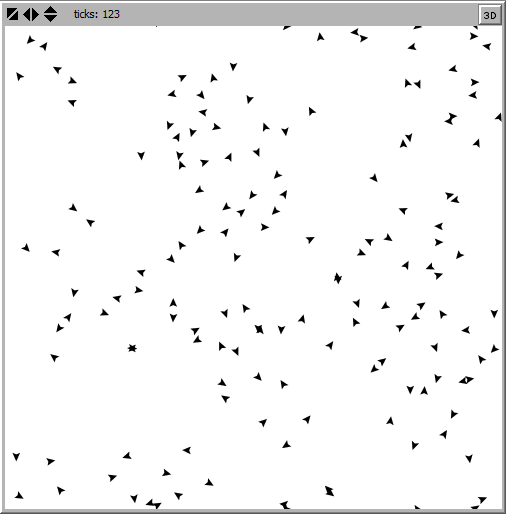
\includegraphics[width=\linewidth]{nomatch.png}
  \caption{No Match}
  
  
 
\end{figure}

This figure shows that the agents are moving individually without maintaining any sequence. However they are moving here and there as per their wish with following the rules of the model.



\begin{figure}[H]
  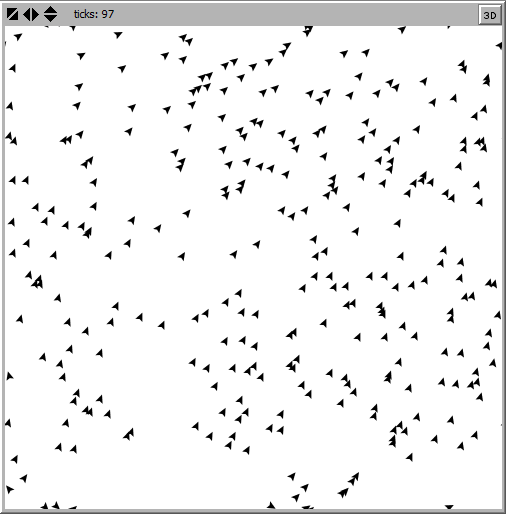
\includegraphics[width=\linewidth]{boxna.png}
  \caption{No Box}
\end{figure}


This figure shows that the agents are moving individually without any limitation within the world. They are moving here and there with following the rules of the model.
 



\begin{figure}[H]
  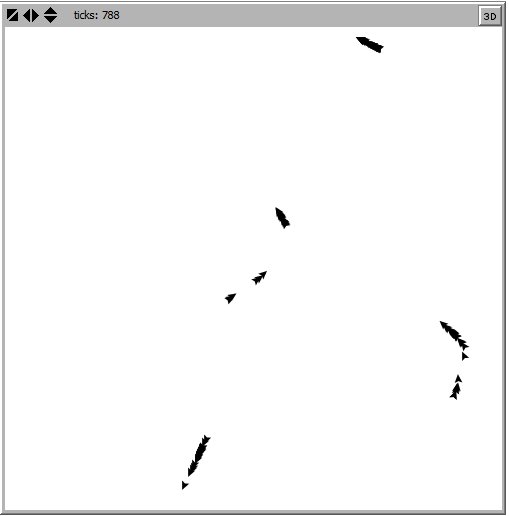
\includegraphics[width=\linewidth]{oneline.png}
  \caption{One Line}
 
\end{figure}

This figure shows that the agents are moving following a single line . They are following each others in a single line.


\begin{figure}[H]
  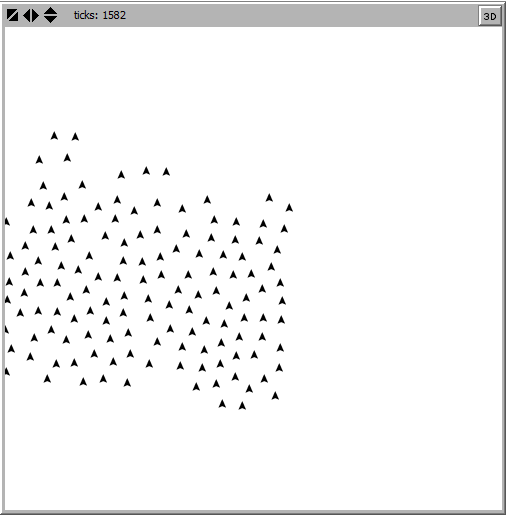
\includegraphics[width=\linewidth]{same.png}
  \caption{Same Direction}
 
\end{figure}

This figure shows that the agents are moving towards the same direction. They are moving into the same direction of the world.


\section{Conclusion}
This report on Couzin Model's modified behavior actually shows us the behavior of animals on different collective values . It indicates some interesting changes that can be related with the real life scenario as well. It helps us to understand the animal behaviors in different atmosphere and conditions. 


\end{document}